\documentclass[tikz,border=2pt]{standalone}
\usepackage{amsmath,amssymb}
\usepackage{tikz}
\usetikzlibrary{arrows.meta}

\begin{document}
% Higher-order partials arise by differentiating again and again, one variable at a time:
% the tree for f(x, y) up to order three (branches: differentiate w.r.t. x or y).
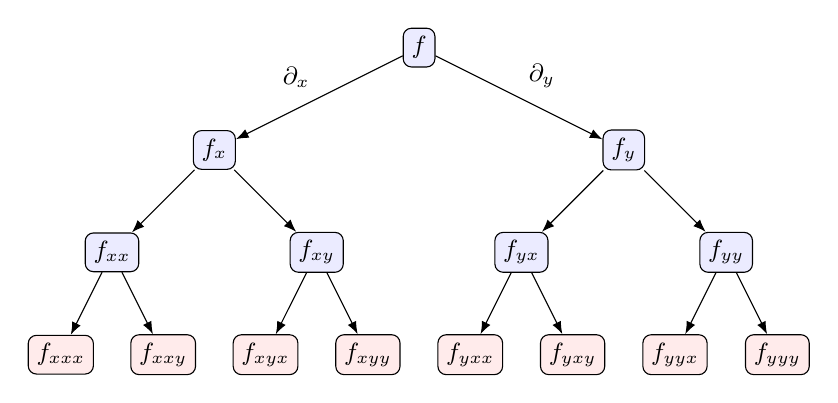
\begin{tikzpicture}[every node/.style={font=\small}, >={Latex[length=1.6mm]}, lvl/.style={draw, rounded corners=3pt, fill=blue!8, inner sep=3pt}]
	\node[lvl] (f) at (0,0) {$f$};
	\node[lvl] (x) at (-2.6,-1.3) {$f_x$};
	\node[lvl] (y) at (2.6,-1.3) {$f_y$};
	\node[lvl] (xx) at (-3.9,-2.6) {$f_{xx}$};
	\node[lvl] (xy) at (-1.3,-2.6) {$f_{xy}$};
	\node[lvl] (yx) at (1.3,-2.6) {$f_{yx}$};
	\node[lvl] (yy) at (3.9,-2.6) {$f_{yy}$};
	\node[lvl, fill=red!8] (xxx) at (-4.55,-3.9) {$f_{xxx}$};
	\node[lvl, fill=red!8] (xxy) at (-3.25,-3.9) {$f_{xxy}$};
	\node[lvl, fill=red!8] (xyx) at (-1.95,-3.9) {$f_{xyx}$};
	\node[lvl, fill=red!8] (xyy) at (-0.65,-3.9) {$f_{xyy}$};
	\node[lvl, fill=red!8] (yxx) at (0.65,-3.9) {$f_{yxx}$};
	\node[lvl, fill=red!8] (yxy) at (1.95,-3.9) {$f_{yxy}$};
	\node[lvl, fill=red!8] (yyx) at (3.25,-3.9) {$f_{yyx}$};
	\node[lvl, fill=red!8] (yyy) at (4.55,-3.9) {$f_{yyy}$};
	\draw[->] (f) -- (x) node[midway, above left] {$\partial_x$};
	\draw[->] (f) -- (y) node[midway, above right] {$\partial_y$};
	\draw[->] (x) -- (xx); \draw[->] (x) -- (xy); \draw[->] (y) -- (yx); \draw[->] (y) -- (yy);
	\draw[->] (xx) -- (xxx); \draw[->] (xx) -- (xxy); \draw[->] (xy) -- (xyx); \draw[->] (xy) -- (xyy);
	\draw[->] (yx) -- (yxx); \draw[->] (yx) -- (yxy); \draw[->] (yy) -- (yyx); \draw[->] (yy) -- (yyy);
\end{tikzpicture}
\end{document}
